
\documentclass[aspectratio=169,14pt]{beamer}
\usetheme{default}\usecolortheme{default}\setbeamertemplate{navigation symbols}{}
\setbeamertemplate{footline}{\hfill{\scriptsize\color{covermuted}\insertframenumber/\inserttotalframenumber}\hspace{0.4cm}\vspace{0.15cm}}
\usepackage{fontspec}\usepackage{xeCJK}\setCJKmainfont{PingFang SC}[BoldFont=PingFang SC Semibold]\setmainfont{Helvetica Neue}[BoldFont=Helvetica Neue Bold]
\usepackage{xcolor}\usepackage{tikz}\usepackage{graphicx}\usepackage{fontawesome5}\usetikzlibrary{positioning,calc,arrows.meta,shadows}
\definecolor{bgmain}{RGB}{238,243,252}\definecolor{panel}{RGB}{238,244,255}\definecolor{factbg}{RGB}{246,242,235}\definecolor{coverprimary}{HTML}{2563EB}\definecolor{coveraccent}{HTML}{00A884}\definecolor{coverwarning}{HTML}{F59E0B}\definecolor{coverdark}{HTML}{1F2937}\definecolor{covermuted}{HTML}{64748B}\definecolor{titlecolor}{RGB}{30,30,30}\definecolor{muteddark}{RGB}{72,86,115}\definecolor{bluepanel}{RGB}{226,237,255}\definecolor{greenpanel}{RGB}{225,246,237}\definecolor{amberpanel}{RGB}{255,244,222}\definecolor{purplepanel}{RGB}{239,231,255}\setbeamercolor{background canvas}{bg=bgmain}
\newcommand{\plainbar}{\begin{tikzpicture}[remember picture, overlay]\fill[coverdark, opacity=0.07] (current page.south west) rectangle ([yshift=0.4cm]current page.south east);\draw[coveraccent, opacity=0.45, line width=0.8pt] ([yshift=0.4cm]current page.south west) -- ([yshift=0.4cm]current page.south east);\end{tikzpicture}}
\newcommand{\deckbackground}{\begin{tikzpicture}[remember picture, overlay]\fill[coverprimary!8] (current page.north west) rectangle (current page.south east);\fill[coverprimary!14] (current page.north west) ++(1.55,-1.35) circle (2.45cm);\fill[coveraccent!12] (current page.south east) ++(-1.9,1.45) circle (2.70cm);\fill[coverwarning!12] (current page.north east) ++(-2.9,-1.8) circle (0.85cm);\foreach \x in {-0.2,0.8,...,16.2} {\draw[coverprimary, opacity=0.045, line width=0.25pt] ([xshift=\x cm]current page.south west) -- ([xshift=\x cm]current page.north west);}\foreach \y in {-0.2,0.7,...,9.3} {\draw[coverprimary, opacity=0.04, line width=0.25pt] ([yshift=\y cm]current page.south west) -- ([yshift=\y cm]current page.south east);}\draw[coveraccent, opacity=0.38, line width=1.1pt] ([xshift=0.35cm,yshift=7.72cm]current page.south west) -- ++(3.25,0) -- ++(0.45,-0.45) -- ++(2.0,0);\draw[coverprimary, opacity=0.24, line width=1.0pt] ([xshift=9.35cm,yshift=8.25cm]current page.south west) -- ++(2.3,0) -- ++(0.55,-0.55) -- ++(3.2,0);\fill[coverdark, opacity=0.07] (current page.south west) rectangle ([yshift=0.42cm]current page.south east);\end{tikzpicture}}
\newcommand{\sectiontitle}[2]{\vspace{-0.52cm}\begin{center}{\fontsize{20}{24}\selectfont\bfseries\color{titlecolor} #1}\\[2pt]{\fontsize{9}{11}\selectfont\itshape\color{muteddark} #2}\end{center}\vspace{0.12cm}}
\newcommand{\portraitbox}[2]{\begin{tikzpicture}\node[draw=coverprimary!28, line width=0.7pt, fill=white, rounded corners=3pt, inner sep=2.5pt, drop shadow={shadow xshift=0.5pt, shadow yshift=-0.5pt, opacity=0.12}] {\includegraphics[width=2.4cm,height=2.9cm,keepaspectratio]{#1}};\end{tikzpicture}{\par\vspace{1pt}\fontsize{6.5}{7.5}\selectfont\color{covermuted} #2\par}}
\newcommand{\personslide}[9]{\begin{frame}\plainbar\vspace{-0.45cm}\begin{center}{\fontsize{22}{26}\selectfont\bfseries\color{coverdark} #1}\\[2pt]{\fontsize{9.5}{11.5}\selectfont\color{muteddark} #2}\end{center}\vspace{0.15cm}\begin{columns}[c]\begin{column}{0.22\textwidth}\centering #3\end{column}\begin{column}{0.28\textwidth}\begin{tikzpicture}\node[fill=greenpanel, rounded corners=4pt, inner xsep=6pt, inner ysep=5pt, text width=3.8cm, align=left] {{\fontsize{7}{8.5}\selectfont\bfseries\color{coveraccent!70!black} 获奖}\enspace{\fontsize{7}{8.5}\selectfont\color{coverdark!85} #4}\\[2.5pt]{\fontsize{7}{8.5}\selectfont\bfseries\color{coveraccent!70!black} 生卒}\enspace{\fontsize{7}{8.5}\selectfont\color{coverdark!85} #5}\\[2.5pt]{\fontsize{7}{8.5}\selectfont\bfseries\color{coveraccent!70!black} 身份}\enspace{\fontsize{7}{8.5}\selectfont\color{coverdark!85} #6}\\[2.5pt]{\fontsize{7}{8.5}\selectfont\bfseries\color{coveraccent!70!black} 机构}\enspace{\fontsize{7}{8.5}\selectfont\color{coverdark!85} #7}};\end{tikzpicture}\end{column}\begin{column}{0.48\textwidth}\begin{tikzpicture}\node[draw=coverprimary!35, fill=bluepanel, rounded corners=5pt, inner sep=7pt, text width=6.6cm, anchor=north west] at (0,0) {{\fontsize{8.6}{10.2}\selectfont\bfseries\color{coverprimary!82!black} 核心贡献}\\[3pt]{\fontsize{7.4}{9.2}\selectfont\color{coverdark!84} #8\\[3pt]\textbf{一句话：} #9}};\end{tikzpicture}\end{column}\end{columns}\end{frame}}

\begin{document}
\begin{frame}[plain]
\deckbackground
\begin{tikzpicture}[remember picture, overlay]
  \node[anchor=center, font=\fontsize{28}{34}\selectfont\bfseries, text=coverdark] at ([yshift=2.05cm]current page.center) {沃尔夫数学奖人物谱系};
  \node[anchor=center, font=\fontsize{15}{19}\selectfont, text=coverprimary!82!black] at ([yshift=0.86cm]current page.center) {第10集 \enspace·\enspace 群论、组合数学与计算};
  \node[anchor=center, font=\fontsize{12}{16}\selectfont\bfseries, text=coveraccent!76!black] at ([yshift=0.10cm]current page.center) {Groups · Combinatorics · Computation · Cryptography};
  \draw[coveraccent, line width=1.4pt] ([yshift=-1.02cm, xshift=-4.55cm]current page.center) -- ([yshift=-1.02cm, xshift=4.55cm]current page.center);
  \node[anchor=center] at ([yshift=-1.90cm]current page.center) {\begin{tikzpicture}\node[rounded corners=8pt, fill=coverprimary!10, inner sep=4pt, minimum height=1.2em, font=\scriptsize\bfseries, text=coverprimary!85!black] at (-5.30,0) {Erdős};\node[rounded corners=8pt, fill=coverprimary!10, inner sep=4pt, minimum height=1.2em, font=\scriptsize\bfseries, text=coverprimary!85!black] at (-3.53,0) {Thompson};\node[rounded corners=8pt, fill=coverprimary!10, inner sep=4pt, minimum height=1.2em, font=\scriptsize\bfseries, text=coverprimary!85!black] at (-1.77,0) {Tits};\node[rounded corners=8pt, fill=coverprimary!10, inner sep=4pt, minimum height=1.2em, font=\scriptsize\bfseries, text=coverprimary!85!black] at (0.00,0) {Aschbacher};\node[rounded corners=8pt, fill=coverprimary!10, inner sep=4pt, minimum height=1.2em, font=\scriptsize\bfseries, text=coverprimary!85!black] at (1.77,0) {Lovász};\node[rounded corners=8pt, fill=coverprimary!10, inner sep=4pt, minimum height=1.2em, font=\scriptsize\bfseries, text=coverprimary!85!black] at (3.53,0) {Alon};\node[rounded corners=8pt, fill=coverprimary!10, inner sep=4pt, minimum height=1.2em, font=\scriptsize\bfseries, text=coverprimary!85!black] at (5.30,0) {Shamir};\end{tikzpicture}};
\end{tikzpicture}
\end{frame}
\begin{frame}
\plainbar
\sectiontitle{群论、组合数学与计算}{Groups · Combinatorics · Computation · Cryptography}
\begin{center}\begin{tikzpicture}
  \node[draw=coverprimary!45, fill=bluepanel, rounded corners=5pt, inner sep=8pt, text width=11.2cm, align=left] at (0,1.05) {{\fontsize{8.3}{10}\selectfont\bfseries\color{coverprimary!80!black} 本集主线}\\[3pt]{\fontsize{7.4}{9.2}\selectfont\color{coverdark!84} 本集从组合数学的问题风格讲到有限群分类、建筑理论、图论、组合优化、密码学与理论计算，展现离散数学如何成为现代数学和计算世界的共同语言。}};
  \node[draw=coverwarning!60, fill=amberpanel, rounded corners=5pt, inner sep=7pt, text width=11.2cm, align=center] at (0,-1.45) {{\fontsize{8.0}{9.8}\selectfont\bfseries\color{coverwarning!62!black} 开场问题}\\[-1pt]{\fontsize{7.4}{9}\selectfont\color{coverdark!82} 有限对象为什么会如此复杂？图、群和算法如何支撑现代计算与密码安全？}};
\end{tikzpicture}\end{center}
\end{frame}
\begin{frame}
\plainbar
\sectiontitle{人物路线图}{从早期奠基到现代前沿}
\begin{center}
\begin{tikzpicture}[milestone/.style={draw=coverprimary!45, fill=panel, rounded corners=4pt, inner xsep=4.0pt, inner ysep=5pt, align=center, font=\fontsize{5.9}{7.2}\selectfont\bfseries}, arrow/.style={-{Stealth}, draw=coveraccent, line width=0.7pt}]
\node[milestone, fill=bluepanel] (m0) at (-5.50,1.0) {1983/84\\Erdős\\组合};
\node[milestone, fill=greenpanel] (m1) at (-3.67,1.0) {1992\\Thompson\\有限群};
\node[milestone, fill=amberpanel] (m2) at (-1.83,1.0) {1993\\Tits\\建筑};
\node[milestone, fill=purplepanel] (m3) at (0.00,1.0) {2012\\Aschbacher\\分类};
\node[milestone, fill=bluepanel] (m4) at (1.83,1.0) {1999\\Lovász\\图论};
\node[milestone, fill=greenpanel] (m5) at (3.67,1.0) {2024\\Alon\\组合};
\node[milestone, fill=amberpanel] (m6) at (5.50,1.0) {2024\\Shamir\\密码};
\draw[arrow] (m0) -- (m1);
\draw[arrow] (m1) -- (m2);
\draw[arrow] (m2) -- (m3);
\draw[arrow] (m3) -- (m4);
\draw[arrow] (m4) -- (m5);
\draw[arrow] (m5) -- (m6);
  \node[draw=coverprimary!38, fill=white, rounded corners=5pt, inner sep=7pt, text width=11.4cm, align=left] at (0,-1.25) {{\fontsize{8.0}{9.8}\selectfont\bfseries\color{coverprimary!80!black} 叙事线}\\[-1pt]{\fontsize{7.2}{8.8}\selectfont\color{coverdark!82} 从 Erdős 的问题文化，到 Thompson、Tits、Aschbacher 的群论大工程，再到 Lovász、Alon、Shamir 连接图论、算法与密码，本集展示离散数学如何从纸面结构进入计算时代。}};
\end{tikzpicture}\end{center}
\end{frame}
\begin{frame}
\plainbar
\sectiontitle{本集的四个关键词}{观众需要记住的结构性线索}
\begin{columns}[T]
\begin{column}{0.49\textwidth}\begin{tikzpicture}
\node[draw=coverprimary!45, fill=bluepanel, rounded corners=5pt, inner sep=7pt, text width=6.0cm, anchor=north west] at (0,0) {{\fontsize{8.5}{10}\selectfont\bfseries\color{coverprimary!80!black} 1. 分类}\\[2pt]{\fontsize{7.3}{8.8}\selectfont\color{coverdark!82} 有限单群分类说明，离散对象也可能需要百科全书级的结构理论。}};
\node[draw=coverprimary!45, fill=greenpanel, rounded corners=5pt, inner sep=7pt, text width=6.0cm, anchor=north west] at (0,-2.25) {{\fontsize{8.5}{10}\selectfont\bfseries\color{coveraccent!70!black} 2. 图与优化}\\[2pt]{\fontsize{7.3}{8.8}\selectfont\color{coverdark!82} 图论把关系网络转化为可证明、可计算、可优化的数学对象。}};
\end{tikzpicture}\end{column}
\begin{column}{0.49\textwidth}\begin{tikzpicture}
\node[draw=coverprimary!45, fill=amberpanel, rounded corners=5pt, inner sep=7pt, text width=6.0cm, anchor=north west] at (0,0) {{\fontsize{8.5}{10}\selectfont\bfseries\color{coverwarning!62!black} 3. 概率方法}\\[2pt]{\fontsize{7.3}{8.8}\selectfont\color{coverdark!82} 随机选择常常能证明确定性结构存在，这是现代组合数学的核心思想。}};
\node[draw=coverprimary!45, fill=purplepanel, rounded corners=5pt, inner sep=7pt, text width=6.0cm, anchor=north west] at (0,-2.25) {{\fontsize{8.5}{10}\selectfont\bfseries\color{coverprimary!74!black} 4. 密码计算}\\[2pt]{\fontsize{7.3}{8.8}\selectfont\color{coverdark!82} 数论、复杂性和算法共同支撑现代密码学。}};
\end{tikzpicture}\end{column}
\end{columns}
\end{frame}
\personslide
  {Paul Erdős}
  {保罗·埃尔德什：组合数学与图论的流浪大师}
  {\portraitbox{images/Erdos.jpg}{Photo: Wikipedia}}
  {1983/84（70岁）}
  {1913--1996}
  {匈牙利}
  {Hungarian Academy of Sciences}
  {Erdős 在组合数学、图论、数论和概率方法中贡献巨大，以超高产论文和广泛合作闻名，塑造了现代离散数学的问题风格。}
  {他把组合数学变成一门充满深问题和强方法的现代学科。}
\personslide
  {John G. Thompson}
  {约翰·汤普森：有限群分类的关键推手}
  {\portraitbox{images/Thompson.jpg}{Photo: Wikipedia}}
  {1992（60岁）}
  {1932--}
  {美国}
  {University of Cambridge}
  {Thompson 与 Feit 证明奇阶定理，深刻推动有限单群分类。他获 1970 年菲尔兹奖和 2008 年阿贝尔奖。}
  {有限群分类这座大工程，离不开他的决定性突破。}
\personslide
  {Jacques Tits}
  {雅克·蒂茨：建筑理论与群的几何}
  {\portraitbox{images/Tits.jpg}{Photo: Wikipedia}}
  {1993（63岁）}
  {1930--2021}
  {比利时/法国}
  {Collège de France}
  {Tits 建立建筑理论和 Tits 系，把群论、几何和代数结构联系起来；2008 年与 Thompson 同获阿贝尔奖。}
  {他让抽象群拥有可以被看见和操作的几何骨架。}
\personslide
  {Michael Aschbacher}
  {迈克尔·阿施巴赫：有限单群分类的完成者之一}
  {\portraitbox{images/Aschbacher.jpg}{Photo: Wikipedia}}
  {2012（67岁）}
  {1944--}
  {美国}
  {Caltech}
  {Aschbacher 在有限群论中贡献核心，尤其与有限单群分类的完成和局部分析方法密切相关。}
  {他代表了大型分类工程中最精密、最艰苦的一环。}
\personslide
  {László Lovász}
  {拉兹洛·洛瓦兹：图论与组合优化}
  {\portraitbox{images/Lovasz.jpg}{Photo: Wikipedia}}
  {1999（51岁）}
  {1948--}
  {匈牙利}
  {Eötvös Loránd University / Yale}
  {Lovász 在组合数学、图论、组合优化和算法理论上贡献奠基，LLL 算法等工作影响理论计算机科学；2021 年获阿贝尔奖。}
  {他把图论从离散对象推进为算法和优化的核心语言。}
\personslide
  {Noga Alon}
  {诺加·阿隆：概率方法与极值组合}
  {\portraitbox{images/Alon.jpg}{Photo: Wikipedia}}
  {2024（67岁）}
  {1956--}
  {以色列}
  {Tel Aviv University}
  {Alon 在组合数学和图论中贡献深远，包括组合 Nullstellensatz、扩展图和概率方法。}
  {他展示了随机方法如何解决确定性的组合问题。}
\personslide
  {Adi Shamir}
  {阿迪·沙米尔：密码学与计算复杂性}
  {\portraitbox{images/Shamir.jpg}{Photo: Wikipedia}}
  {2024（71岁）}
  {1952--}
  {以色列}
  {Weizmann Institute of Science}
  {Shamir 是 RSA 加密算法共同发明者之一，并在密码学、复杂性和理论计算中贡献突出；2002 年获图灵奖。}
  {他把数论和计算复杂性变成现代数字安全的基础。}
\begin{frame}
\plainbar
\sectiontitle{第10集的主线}{群论、组合数学与计算}
\begin{center}\begin{tikzpicture}[block/.style={draw=coverprimary!42, fill=white, rounded corners=5pt, inner sep=6pt, text width=3.0cm, align=center, font=\fontsize{7.0}{8.5}\selectfont}, arrow/.style={->, draw=coveraccent, line width=0.85pt}]
  \node[block, fill=bluepanel] (a) at (-4.9,1.25) {\textbf{起点}\\基础语言}; \node[block, fill=greenpanel] (b) at (-1.65,1.25) {\textbf{工具}\\结构方法}; \node[block, fill=amberpanel] (c) at (1.65,1.25) {\textbf{突破}\\核心定理}; \node[block, fill=purplepanel] (d) at (4.9,1.25) {\textbf{影响}\\跨域应用};
  \draw[arrow] (a) -- (b); \draw[arrow] (b) -- (c); \draw[arrow] (c) -- (d);
  \node[draw=coverwarning!65, fill=factbg, rounded corners=5pt, inner sep=7pt, text width=11.1cm, align=left] at (0,-1.35) {{\fontsize{8.0}{9.8}\selectfont\bfseries\color{coverwarning!62!black} 一句话总结}\\[-1pt]{\fontsize{7.4}{9}\selectfont\color{coverdark!84} 从 Erdős 的问题文化，到 Thompson、Tits、Aschbacher 的群论大工程，再到 Lovász、Alon、Shamir 连接图论、算法与密码，本集展示离散数学如何从纸面结构进入计算时代。}};
\end{tikzpicture}\end{center}
\end{frame}
\begin{frame}
\plainbar
\sectiontitle{下一步}{专题系列衔接}
\begin{center}\begin{tikzpicture}
  \node[draw=coverwarning!60, fill=coverwarning!12, rounded corners=5pt, inner sep=7pt, text width=10.5cm, align=center] at (0,1.4) {{\fontsize{8.4}{10}\selectfont\bfseries\color{coverwarning!65!black} 下一集：动力系统与遍历理论}\\[-1pt]{\fontsize{7.4}{9}\selectfont\color{coverdark!80} 从离散结构进入运动、混沌、遍历和刚性。}};
  \node[draw=coverprimary!45, fill=bluepanel, rounded corners=5pt, inner sep=8pt, text width=10.5cm, align=center] at (0,-1.35) {{\fontsize{10.5}{12.8}\selectfont\bfseries\color{coverprimary!82!black} Jürgen Moser、Vladimir Arnold、Yakov Sinai、Hillel Furstenberg、Grigory Margulis}};
\end{tikzpicture}\end{center}
\end{frame}
\end{document}
